\section{Wireless Networks}
\subsection{Wireless}
\begin{itemize}[nosep]
    \item Today: wireless networking truly ubiquitous
          \begin{itemize}[nosep]
              \item 802.11, 3G, 4G, 5G, WiMAX, Bluetooth, RFID, \dots
              \item Sensor networks, Internet of Things (IoT)
              \item Some new computers have no \emph{wired} networking
          \end{itemize}
    \item What's behind the scenes?
\end{itemize}

\subsection{Wireless is different}
\begin{itemize}[nosep]
    \item Signals sent by the sender don't always reach the receiver intact
          \begin{itemize}[nosep]
              \item Varies with \emph{space}: attenuation, multipath
              \item Varies with \emph{time}: conditions change, intereference, mobility
          \end{itemize}
    \item \emph{Distributed}: sender doesn't know what happens at receiver
    \item Wireless medium is inherently \emph{shared}
          \begin{itemize}[nosep]
              \item No easy way out with switches
          \end{itemize}
\end{itemize}

\subsection{Implications}
\begin{itemize}[nosep]
    \item Different mechanisms needed
    \item Physical layer
          \begin{itemize}[nosep]
              \item Different knobs: antennas, transmission power, encodings
          \end{itemize}
    \item Link Layer
          \begin{itemize}[nosep]
              \item Distributed medium access protocols
              \item Topology awareness
          \end{itemize}
    \item Network, Transport Layers
          \begin{itemize}[nosep]
              \item Routing, forwarding
          \end{itemize}
    \item Most advances \emph{do not} abstract away the physical and link layers
\end{itemize}

\subsection{Interference}
\begin{itemize}[nosep]
    \item External sources
          \begin{itemize}[nosep]
              \item e.g. 2.4\si{GHz} unlicensed ISM band
              \item 802.11
              \item 802.15.4 (ZigBee), 802.15.1 (Bluetooth)
              \item 2.4\si{GHz} phones
              \item Microwave ovens
          \end{itemize}
    \item Internal sources
          \begin{itemize}[nosep]
              \item Nodes in the same network/protocol can (and do) interfere
          \end{itemize}
    \item Multipath
          \begin{itemize}[nosep]
              \item Self-interference (destructive)
          \end{itemize}
\end{itemize}

\subsection{Link Layer}
\begin{itemize}[nosep]
    \item Medium Access Control
          \begin{itemize}[nosep]
              \item Should give 100\% if one user
              \item Should be efficient and fair if more users
          \end{itemize}
    \item Ethernet uses CSMA/CD
          \begin{itemize}[nosep]
              \item Can we use CD here?
          \end{itemize}
    \item No! Collision happens at the receiver
    \item Protocls try to \emph{avoid} collision in the first place
\end{itemize}

\subsection{Hidden Terminals}
\begin{figure}[H]
    \tikzsetnextfilename{hidden-terminals}
    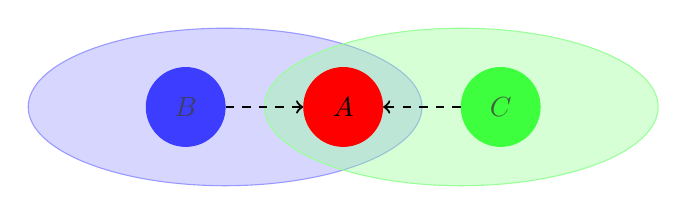
\begin{tikzpicture}[every node/.style={circle,draw,fill,minimum size=1cm}]
        \node[blue] at (-2, 0) (b) {\textcolor{black}{$B$}};
        \node[green] at (2, 0) (c) {\textcolor{black}{$C$}};

        \draw[fill,blue!40!white,fill opacity=0.4] ([xshift=0.5cm]b) ellipse (2.5 and 1);
        \draw[fill,green!40!white,fill opacity=0.4] ([xshift=-0.5cm]c) ellipse (2.5 and 1);

        \node[red] at (0, 0)   (a) {\textcolor{black}{$A$}};
        \draw[->,dashed,thick] (b) -- (a);
        \draw[->,dashed,thick] (c) -- (a);
    \end{tikzpicture}
\end{figure}
\begin{itemize}[nosep]
    \item $A$ can hear $B$ and $C$
    \item $B$ and $C$ can't hear each other
    \item They both interfere at $A$
    \item $B$ is a \emph{hidden terminal} to $C$, and vice-versa.
    \item \emph{Carrier sense at sender is useless}
\end{itemize}

\subsection{Exposed Terminals}
\begin{figure}[H]
    \tikzsetnextfilename{exposed-terminals}
    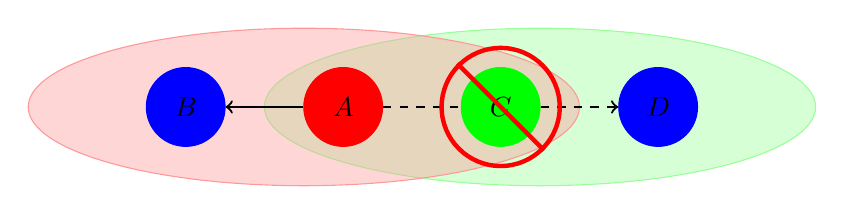
\begin{tikzpicture}[every node/.style={circle,draw,fill,minimum size=1cm}]
        \draw[fill,green!40!white,fill opacity=0.4] (2.5,0) ellipse (3.5 and 1);
        \draw[fill,red!40!white,fill opacity=0.4] (-0.5,0) ellipse (3.5 and 1);

        \node[green] at (2, 0) (c) {\textcolor{black}{$C$}};
        \node[red] at (0, 0)   (a) {\textcolor{black}{$A$}};
        \node[blue] at (-2, 0) (b) {\textcolor{black}{$B$}};
        \node[blue] at (4, 0) (d) {\textcolor{black}{$D$}};
        \draw[->,thick] (a) -- (b);
        \draw[->,dashed,thick] (a) -- (c) -- (d);

        \node[circle,red,minimum size=1.5cm,ultra thick,fill=none,draw] at (c) (s) {};
        \draw[red,ultra thick] (s.south east) -- (s.north west);
    \end{tikzpicture}
\end{figure}
\begin{itemize}[nosep]
    \item $A$ transmits to $B$
    \item $C$ hears the transmission, backs off, even though $D$ would hear $C$
    \item They both interfere at $A$
    \item $C$ is an \emph{exposed terminal} to $A$'s transmission
\end{itemize}

\subsection{Key points}
\begin{itemize}[nosep]
    \item No global view of collision
          \begin{itemize}[nosep]
              \item Different receivers hear different senders
              \item Different senders reach different receivers
          \end{itemize}
    \item Collisions happen at the \emph{receiver}
    \item Goals of a MAC protocol
          \begin{itemize}[nosep]
              \item Detect if receiver can hear sender
              \item Tell senders who might interfere with receiver to shut up
          \end{itemize}
\end{itemize}

\subsection{RTS/CTS}
\begin{itemize}[nosep]
    \item Idea: transmitter can check availabilty of channel at receiver
    \item Before every transmission
          \begin{itemize}[nosep]
              \item Sender sends an RTS (Request-to-Send)
              \item Contains length of data (in \emph{time} units)
              \item Receiver sends a CTS (Clear-to-Send)
              \item Sender sends data
              \item Receiver sends ACK after transmission
          \end{itemize}
    \item If you don't hear a CTS, assume collision
    \item If you hear a CTS for someone else, shut up
\end{itemize}

\begin{figure}[H]
    \tikzsetnextfilename{RTS}
    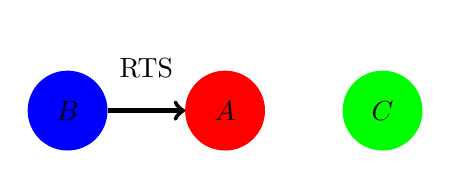
\begin{tikzpicture}[every node/.style={circle,draw,fill,minimum size=1cm}]
        \node[red] at (0, 0)   (a) {\textcolor{black}{$A$}};
        \node[blue] at (-2, 0) (b) {\textcolor{black}{$B$}};
        \node[green] at (2, 0) (c) {\textcolor{black}{$C$}};

        \draw[ultra thick,->] (b) -- (a) node[above,pos=0.5,draw=none,fill=none] {RTS};
    \end{tikzpicture}
\end{figure}

\begin{figure}[H]
    \tikzsetnextfilename{CTS}
    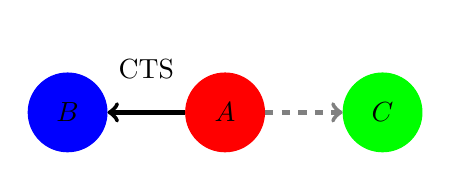
\begin{tikzpicture}[every node/.style={circle,draw,fill,minimum size=1cm}]
        \node[red] at (0, 0)   (a) {\textcolor{black}{$A$}};
        \node[blue] at (-2, 0) (b) {\textcolor{black}{$B$}};
        \node[green] at (2, 0) (c) {\textcolor{black}{$C$}};

        \draw[ultra thick,->] (a) -- (b) node[above,pos=0.5,draw=none,fill=none] {CTS};
        \draw[ultra thick,dashed,->,gray] (a) -- (c);
    \end{tikzpicture}
\end{figure}

\begin{figure}[H]
    \tikzsetnextfilename{rtsdata}
    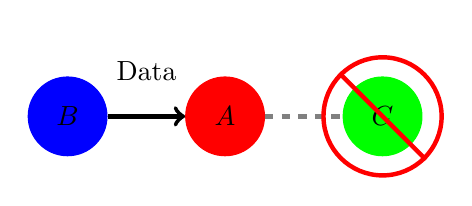
\begin{tikzpicture}[every node/.style={circle,draw,fill,minimum size=1cm}]
        \node[red] at (0, 0)   (a) {\textcolor{black}{$A$}};
        \node[blue] at (-2, 0) (b) {\textcolor{black}{$B$}};
        \node[green] at (2, 0) (c) {\textcolor{black}{$C$}};

        \draw[ultra thick,->] (b) -- (a) node[above,pos=0.5,draw=none,fill=none] {Data};
        \draw[ultra thick,dashed,gray] (a) -- (c);

        \node[red,circle,ultra thick,minimum size=1.5cm,fill=none] at (c) (s) {};
        \draw[red,ultra thick] (s.south east) -- (s.north west);
    \end{tikzpicture}
\end{figure}

\subsection{Benefits of RTS/CTS}
\begin{itemize}[nosep]
    \item Solves hidden terminal problem
    \item Does it?
          \begin{itemize}[nosep]
              \item Control frames can still collide
              \item e.g. can cause CTS to be lost
              \item In practice: reduces hidden terminal problem on data packets
          \end{itemize}
\end{itemize}

\subsection{Drawbacks of RTS/CTS}
\begin{itemize}[nosep]
    \item Overhead is too large for small packets
          \begin{itemize}[nosep]
              \item 3 packets per packet: RTS/CTS/Data (4-22\% for 802.11b)
          \end{itemize}
    \item RTS still goes through CSMA: can be lost
    \item 33\% of IP packets are TCP ACKs
    \item \emph{In practice, WiFi doesn't use RTS/CTS}
\end{itemize}

\subsection{Other MAC Strategies}
\begin{itemize}[nosep]
    \item Time Division Multiplexing (TDMA)
          \begin{itemize}[nosep]
              \item Central controller allocates a time slot for each sender
              \item May be inefficient when not everyone is sending
          \end{itemize}
    \item Frequency Division
          \begin{itemize}[nosep]
              \item Multiplexing two networks on same space
              \item Nodes with two radios (think graph coloring)
              \item Different frquency for upload and download
          \end{itemize}
\end{itemize}

\subsection{Network Layer}
\begin{itemize}[nosep]
    \item What about the network topology?
    \item Almost everything you use is \emph{single hop}!
          \begin{itemize}[nosep]
              \item 802.11 in infrastructure mode
              \item Bluetooh
              \item Cellular networks
              \item WiMax (some 4G Networks)
          \end{itemize}
    \item Why?
          \begin{itemize}[nosep]
              \item Really hard to make multihop wireless efficient
          \end{itemize}
\end{itemize}

\subsection{WiFi Distribution System}
\begin{itemize}[nosep]
    \item 802.11 typically works in \emph{infrastructure mode}
          \begin{itemize}[nosep]
              \item Access points -- fixed noeds on a wired network
          \end{itemize}
    \item Distributed system connects APs
          \begin{itemize}[nosep]
              \item Typically connect to the same Ethernet, use learning bridge to route to nodes' MAC addresses
          \end{itemize}
    \item Association
          \begin{itemize}[nosep]
              \item Node negotiates with AP to get access
              \item Security negotiated as well (WEP, WPA, etc)
              \item Passive or Active
          \end{itemize}
\end{itemize}

\subsection{Wireless Multi-Hop Networks}
\begin{itemize}[nosep]
    \item Some networks are multihop, though!
          \begin{itemize}[nosep]
              \item Ad-hoc networks for emergency areas
              \item Vehicular Networks
              \item Sensor Networks
                    \begin{itemize}[nosep]
                        \item e.g. infrastructure monitoring
                    \end{itemize}
              \item Multihop networking to share Internet access
          \end{itemize}
\end{itemize}

\subsection{What can happen to signals?}
\begin{itemize}[nosep]
    \item Attenuation
          \begin{itemize}[nosep]
              \item Signal power attenuates by $\approx r^2$ factor for omni-directional antennas in a free-space
              \item Exponent depends on type and placement of antennas
                    \begin{itemize}[nosep]
                        \item < 2 for directional antennas
                        \item > 2 if antennas are close to the ground
                    \end{itemize}
          \end{itemize}
\end{itemize}

\subsection{Interference}
\subsection{Multipath}
\begin{itemize}[nosep]
    \item May cause attenuation, destructive intereference
\end{itemize}
\subsection{Many Challenges}
\begin{itemize}[nosep]
    \item Routing
          \begin{itemize}[nosep]
              \item Link estimation
          \end{itemize}
    \item Multihop throughput dropoff
\end{itemize}

\subsection{The Routing Problem}
\begin{figure}[H]
    \tikzsetnextfilename{routing-problem}
    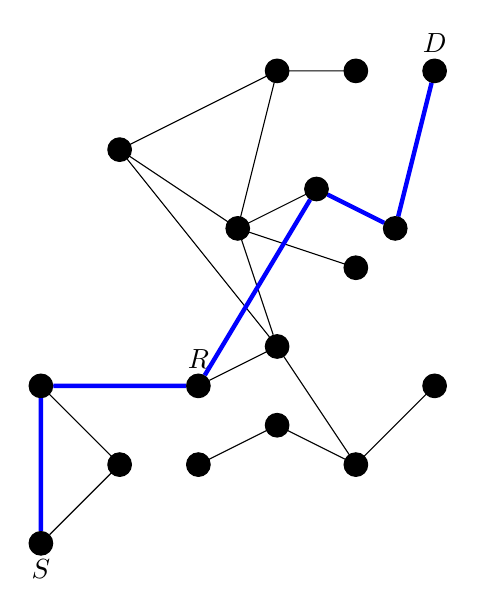
\begin{tikzpicture}[every node/.style={draw,circle,minimum size=0.3cm,inner sep=0,fill}]
        \node[label=below:{$S$}] at (0,0) (s) {};
        \node[label=above:{$R$}] at (2,2) (r) {};
        \draw (s) -- (1,1) node {} -- (0,2) node (step1) {} -- (r) -- (3, 2.5) node (m1) {} -- (4, 1) node (m2) {} -- (5, 2) node {};
        \draw (m2) -- (3, 1.5) node {} -- (2, 1) node {};
        \draw (m1) -- (2.5, 4) node {} -- (4, 3.5) node {};
        \draw (m1) -- (1, 5) node {} -- (3, 6) node {} -- (4, 6) node {};
        \draw (2.5, 4) -- (3.5, 4.5) node (step2) {} -- (4.5, 4) node (step3) {} -- (5, 6) node[label=above:{$D$}] (d) {};
        \draw (3,6) -- (2.5,4) -- (1,5);
        \draw[blue,ultra thick] (s) -- (step1) -- (r) -- (step2) -- (step3) -- (d);
    \end{tikzpicture}
\end{figure}
\begin{itemize}[nosep]
    \item Find a route from $S$ to $D$
    \item Topology can be very dynamic
\end{itemize}

\subsection{Routing}
\begin{itemize}[nosep]
    \item Routing in ad-hoc networks has had a lot of research
          \begin{itemize}[nosep]
              \item General problem: any-to-any routing
              \item Simplified versions: any-to-one (base station), one-to-any (dissemination)
          \end{itemize}
    \item DV too brittle: inconsistencies can cause loops
    \item DSDV
          \begin{itemize}[nosep]
              \item Destination Sequenced Distance Vector
          \end{itemize}
\end{itemize}

\subsection{DSDV}
\begin{itemize}[nosep]
    \item Charles Perkins (1994)
    \item Avoid loops by using sequence numbers
          \begin{itemize}[nosep]
              \item Each destination increments own sequence
                    \begin{itemize}[nosep]
                        \item Only use \emph{even} numbers
                    \end{itemize}
              \item A node selects a new parent if
                    \begin{itemize}[nosep]
                        \item Newer sequence number or
                        \item Same sequence number and \emph{better} route
                    \end{itemize}
          \end{itemize}
    \item If disconnected, a node increments destination sequence number to next \emph{odd} number!
    \item No loops (only transient loops)
    \item Slow: on some changes, need to wait for root
\end{itemize}
\subsection{Many Others}
\begin{itemize}[nosep]
    \item DSR, AODV: on-demand
    \item Geographic routing: use nodes' physical location and do greedy routing
    \item Virtual coordinates: derive coordinates from topology, use greedy routing
    \item Tree-based routing with on-demand shortcuts
    \item \dots
\end{itemize}